\documentclass[a4paper,10pt]{article} 

\usepackage[utf8]{inputenc}     % UTF-8 Zeichensatz unter Linux -> ansonsten auf "applemac" oder "latin1" (Windows ISO-LANGE-NUMMER) ändern und diese Datei durch einen Konverter jagen ( Entsprechende Tools -> Google )

\usepackage[english]{babel}     % Deutsche Worttrennung, Umlaute etc.
\usepackage[T1]{fontenc}        % Erweiterte Textcodierung (z.B a" -> ä)


\usepackage{textcomp}           % Extra Symbole (Grad Celsius etc.)
\usepackage{amssymb,amsmath}    % Schöne Formeln (AMS = American Mathematical Society)
\usepackage{graphicx}           % Bilder und Seitenränder
\usepackage{subcaption}			% captions for subfigures
\usepackage{booktabs}           % Schönere Tabellen
\usepackage{colortbl}           % Farbige Tabellen

%\usepackage[all]{hypcap}        % Verhaltenskorrektur für hyperref
%\usepackage{url}				% URLs
\usepackage{multirow}			% Tabellen mit mehreren Einträgen/Zeile
%\usepackage{tcolorbox}			% schöne bunte Boxen
\usepackage{mathtools}			% \mathclap für ordentliche \underbrace-			environments
\usepackage{geometry}			% Pagelayout mit \newgeometry, \restoregeometry
\usepackage{float}
\usepackage{wrapfig}
\usepackage{sidecap}			% side captions für Bilder; Befehl: % \begin{SCfigure}
\usepackage{bbm}				% for unity matrix (doublestroke 1) 
%\usepackage{pifont}
\usepackage{enumitem}
\usepackage{siunitx}			% proper SI unit typefacing
\usepackage{nicefrac}			% slanted fractions like 3/5
\usepackage{float}

%===============================%
\usepackage[singlelinecheck=false, figurename=Abb., aboveskip=7pt, belowskip=0pt]{caption}
				% richtet side captions ordentlich ein

%===============================%
%\bibliographystyle{dinat}       % Literaturverzeichnis nach DIN1505

% Change the itemize labels to some other symbol - needs enumitem
% where to look for graphics if they're not found
\graphicspath{{./img/}}

% renew figure and table names
\addto\captionsenglish{%
  \renewcommand{\figurename}{Fig.}%
  \renewcommand{\tablename}{Tab.}
  \renewcommand{\contentsname}{Table of Contents}%
}
% own commands


% bibliography style

\usepackage[numbers]{natbib} %use sort instead of cite
\bibliographystyle{unsrtnat}

%=================Title page===================%
\begin{document}


%==============================================%
%=============BEGIN OF DOCUMENT================%
%==============================================%

\begin{titlepage}
 \begin{center}
	\Large{Advance laboratory class 2}
	\end{center}
	\begin{center}
	 \LARGE{\textbf{FP2 - W and Z boson decay}}
	\end{center}
	
	\begin{center}
	report by: \\
	Marco \textsc{Canteri} \footnote{marco.canteri@student.uibk.ac.at},
	Johannes \textsc{Willi} \footnote{johannes.willi@student.uibk.ac.at},
	\end{center}
	
	\begin{center}
	\vspace{1cm}
	Innsbruck, \today
	\vspace{2cm}
	\end{center}
	
	\begin{center}
	
\includegraphics[scale=0.4]{img/uibk} 
	\end{center}

\end{titlepage}
\begin{abstract}
In this work we have analysed several events from the detector ATLAS in order to identify and study two bosons: W boson and Z boson. The study is divided in three parts: first of all
we looked at 40 events and found a ratio between W and Z decays of $W/Z = 6 \pm 3.5$; second we tried to reconstruct the proton structure starting from 100 events of W boson decays; in the third part we focused on Z boson decays and we obtained a mass of Z of $90.0\pm1.3$ GeV, a particle candidate for Higgs boson of mass $127.8\pm 3.0$ GeV, and a possible Z$'$ boson of mass $1150\pm85$ GeV.
\end{abstract}
\section{Introduction}
In this experiment we look at data from proton-proton-collisions from the Large Hadron Collider (LHC) at CERN, Switzerland. In particular, we are interested in the gauge bosons of the weak force, the W and Z boson. The data we analyse is both from simulated and real events. To analyse it, we use two programs: HYPATIA and MINERVA. These two programs allow the analysis of files provided to us by our supervisor, with features like calculation of invariant mass, graphical representation of particle tracks, charge of a particle etc.
ATLAS is mainly composed in three parts: an innermost tracking chamber that can detect charged particle and can give information about charge, momentum and energy; electromagnetic and hadronic calorimeters where photons, electrons, positrons and hadronic particles leave a deposit of energy; and a muon chamber for detecting muons, which don't stop inside the calorimeters. In addition it is possible to indirectly observe neutrinos by computing the missing transverse momentum. 
The main purpose of this work is to study the gauge particles for weak interaction: Z boson and W boson. Due to the short life of these bosons (around $\SI{E-25}{\second}$, the path to study these particles is by means of decay products. Indeed W and Z bosons can decay in leptons or quarks that have a longer life and can be detected by e.g. ATLAS. We didn't study every possible decay channel, but instead we focused on those which have detectable particles as decay products. For example a W boson can decay in a pair composed of a lepton and neutrino. The easiest particles of W decay to identify in ATLAS are electrons and muons and their respective antiparticles, so the channel we focused on are
\[W^- \to e^- + \overline{\nu}_e \qquad W^- \to \mu^- + \overline{\nu}_\mu\]
\[W^+ \to e^+ + \nu_e \qquad W^+ \to \mu^+ + \nu_\mu. \]
The Z boson decays into a pair of lepton and antilepton in around 10\% of cases, with around 20\% into neutrino and antineutrino and around 70\% into quark-antiquark pairs. Again, since we are dealing with ATLAS events, we search for the easiest decay channels that we can be see in our detector. Those decays are
\[Z \to e^+ + e^- \qquad Z \to \mu^+ + \mu^-.\]
Furthermore, among all the events we also searched for evidence of Higgs boson decays through these decay channels
\[H \to \gamma + \gamma \quad H \to Z+ Z \qquad H \to W^+ + W^-.\]

\section{Excercise 1: W/Z events ratio}
\begin{table}[h]
\centering
\begin{tabular}{cccccc}
 $W\to e\nu$ & $W\to \mu\nu$ & $Z\to ee$ & $Z\to \mu\mu$ & $H\to 4l$ & Background \\
\hline
8 & 10 & 1 & 2 & 0 & 19\\
\hline
\end{tabular}
\caption{\label{tab:table1}Number of events identified in our data. We made no distinction between particles and their antiparticles. Here $l$ means any lepton}
\end{table}
We used HYPATIA in order to analyse $N=40$ simulated events, in table \ref{tab:table1} we reported the number of events that we observed in our data.
The ratio between observed decays of W and Z boson is $ N_W/N_Z = 6\pm 3.5$. As errors of $N_W$ and $N_Z$ we used the standard deviation of the multinomial distribution
\[\sigma_W^2 =  N_W\left(1-\frac{N_W}{N}\right) \qquad \sigma_Z^2 =  N_Z\left(1-\frac{N_Z}{N}\right).\]
Therefore it easy to propagate the error:
\[\sigma(N_W/N_Z) = \frac{N_W}{N_Z}\sqrt{\left(\frac{\sigma_W}{N_W}\right)^2+\left(\frac{\sigma_Z}{N_Z}\right)^2}.\]


\section{Excercise 2: Proton structure}
\begin{table}[h]
\centering\small
\begin{tabular}{cccccc}
 $W^+\to e^+ + \nu_e$ & $W^-\to e^- + \bar{\nu}_e$ & $W^+\to \mu^+ + \nu_\mu$ & $W^-\to \mu^- + \bar{\nu}_\mu$ & $\text{H}\to W^++W^-  $& Background \\
\hline
21 & 9 & 25 & 10 & 3 & 32\\
\hline
\end{tabular}
\caption{\label{tab:table2}Number of events identified in our data}
\end{table}
We analysed 100 events total with the software MINERVA searching for W boson decays. In order to understand the proton structure we needed to distinguish between $W^+$ bosons and $W^-$ bosons, in fact a proton is composed by up and down quarks. Therefore, a $W^+$ is produced by a quark up and a $W^-$ by a quark down. Hence is possible to determine the ratio between quark up and quark down inside a proton by calculating the ratio between a production of a $W^+$ boson and a $W^-$ boson via gluon quark interaction.
In theory, $W^\pm$ bosons are created in two different classes of reactions: via quark-gluon (QG) interactions or via gluon-gluon (GG) interactions. Consider the following matrix: \vspace{0.25cm}

\begin{center}
    \begin{tabular}{l|cc|l}
     Interaction & \multicolumn{2}{|c|}{Process}               & Proportion \\ \hline
    Quark-gluon & $\quad$ A $\quad$ & $\quad$ B $\quad$ & 2/3                     \\
    Gluon-gluon & $\quad$ C $\quad$ & $\quad$ D $\quad$ & 1/3                     \\ \vspace{0.25cm}
    \end{tabular}
\end{center}
where $A, B, C, D$ stand for the following processes
\begin{itemize}
\item A: creation of a $W^+$ boson via quark-gluon interaction
\item B: creation of a $W^-$ boson via quark-gluon interaction
\item C: creation of a $W^+$ boson via gluon-gluon interaction
\item D: creation of a $W^-$ boson via gluon-gluon interaction
\end{itemize} 
and are at first unknown, with the only known constraint being $A + B +C+D=1$. We ultimately want to know the ratio $A/B = R_\pm$, i.e., the ratio of $W^+$ to $W^-$ bosons produced only in QG interactions. From this one can draw conclusions about the inner structure of the proton, in particular about the number of up- to down-quarks. 
However, our experimental data only gives us the coefficients $N_+\equiv A+C$ (the number of $W^+$ bosons) and $N_-\equiv B+D$ (the number of $W^-$ bosons). We can, however, assume that both GG interactions occur equally often, i.e.,
\[C = N_{GG}(W^+) = N_{GG}(W^-) = D = 1/6\]
and thus
\[R_\pm = \frac{N_+ - N_{GG}(W^+)}{N_- - N_{GG}(W^-)}.\]
As can be easly calculated from table \ref{tab:table2}  we have $N_+/N_- = 2.38 \pm 0.62$, which is compatible with \cite{ratio} $1.52 \pm 0.07$. The error is calculated by propagation on the ratio and the error of very event is the standard deviation of the Poisson distribution, such as in the previous section. Via the Excel sheet our supervisor gave us we calculated $R_\pm = 4.16\pm 2.26$, which is within the theoretically expected value of $R_\pm = 2$. The large error margin is due to us being the first group and thus having the smallest data set available.

\section{Excercise 3: Z decays and mass determination}
\begin{figure}[H]
\centering
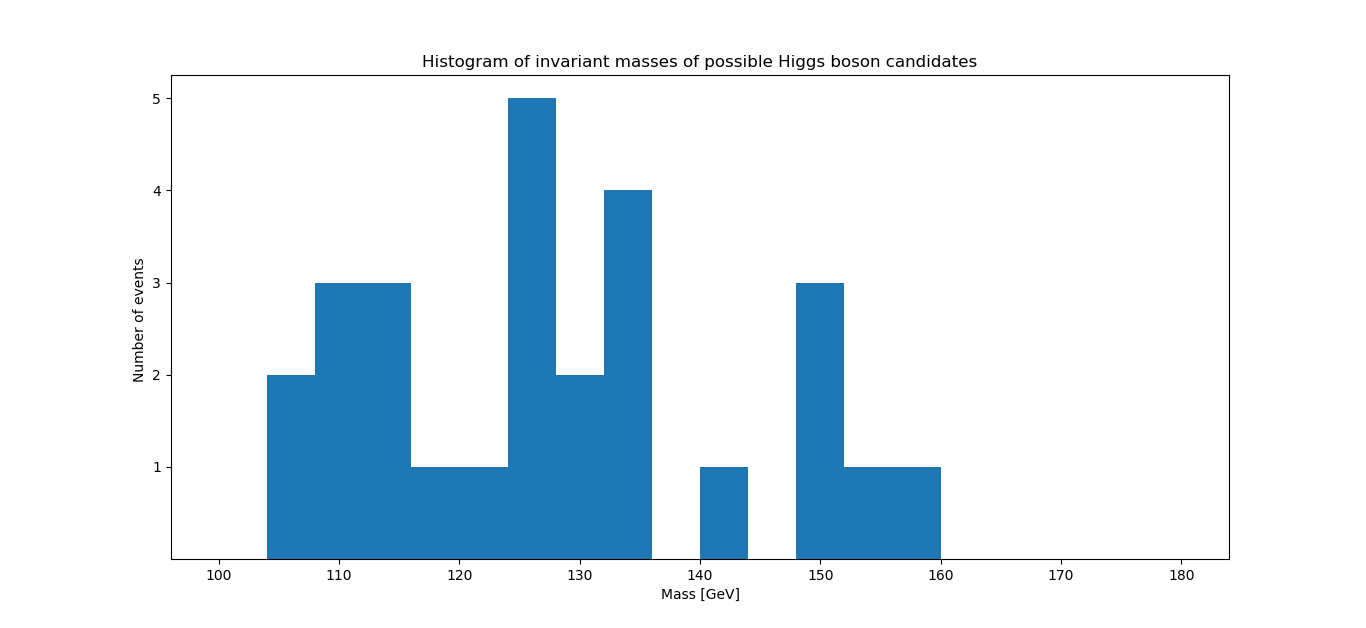
\includegraphics[width =.8\textwidth]{img/higgs}
\caption{Histogram of the invariant masses of possible Higgs boson candidates}\label{higghistogram}
\end{figure}
In order to estimate the mass of the Z boson we analysed 100 events with the software HYPATIA and did the same for the Higgs boson. After the identification of the events, i.e. $Z \to l\bar{l}$, $H\to \gamma\gamma$, and $H\to ZZ\to4l$, we used the Invariant Mass tool to evaluate the mass of the particle decayed. In figure \ref{higghistogram} we plotted an histogram for all the events of possible Higgs candidates. The mean value of the mass is $127.8\pm 3.0$ GeV, where the error is the standard deviation of the data divided by the square root of the number of data. The result is compatible with the literature value \cite{masshiggs} of  $125.09\pm 0.32$ GeV.\\
For the Z boson the data are in figure \ref{Zhistogram}, as can be seen, there is a peak near 90 GeV, which it is what we expected, but there are also some data in the order of 1000 GeV. These data could be candidates for a possible Z$'$ boson. The estimated mass of the Z boson is $90.0\pm1.3$ GeV, while for the possible Z$'$ boson is $1150\pm85$ GeV, with error calculated as for the Higgs boson. The Z mass is compatible with the real value \cite{Zmass} $91.1876 \pm 0.0021$ GeV.\\
Another estimation for the Z mass can be obtained with a Lorentz fit over the histogram, this is depicted in figure \ref{fit}. The fit is done with the function
\[f(x) = \frac{1}{\pi}\frac{\Gamma}{(x-m)^2+\Gamma^2}\]
where $m$ and $\Gamma$ are two parameters to be determined with the fit and they are the x-value for the peak and the half width half maximum of the distribution. The best fit gave us $m = 90.7$ GeV and $\Gamma = 2.1$ GeV.
\begin{figure}[H]
\centering
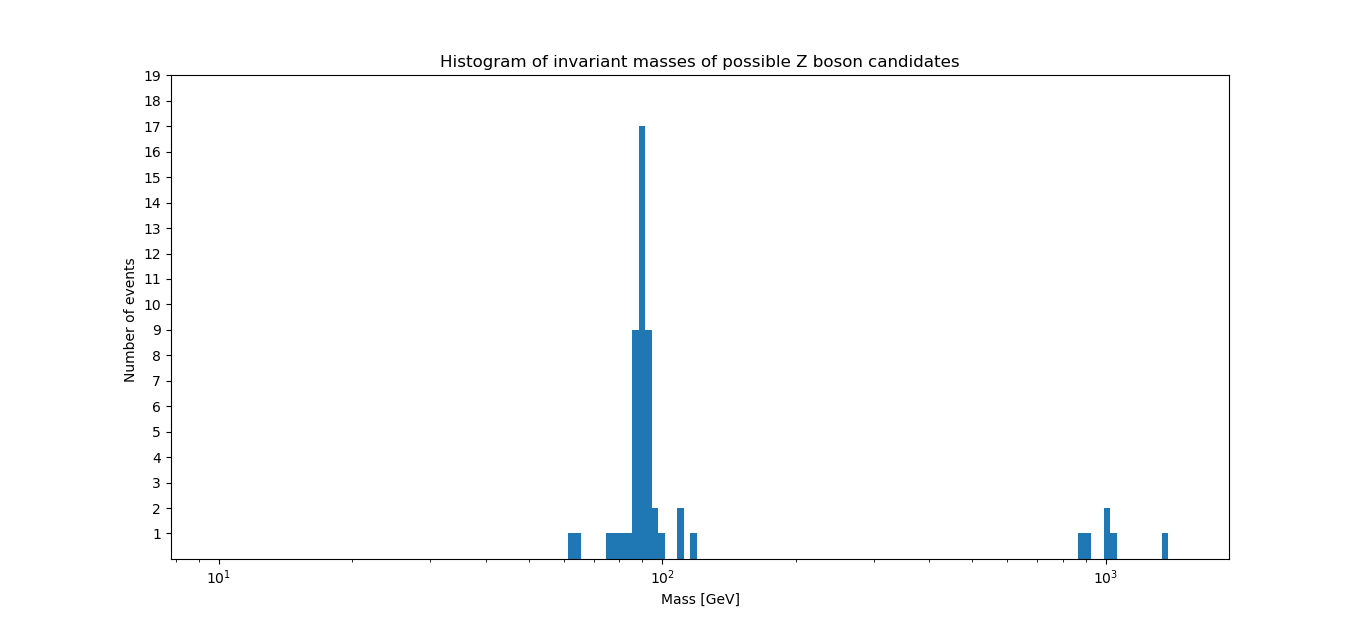
\includegraphics[width =.8\textwidth]{img/Zboson}
\caption{Histogram of the invariant mass of Z decays}\label{Zhistogram}
\end{figure}
\begin{figure}[H]
\centering
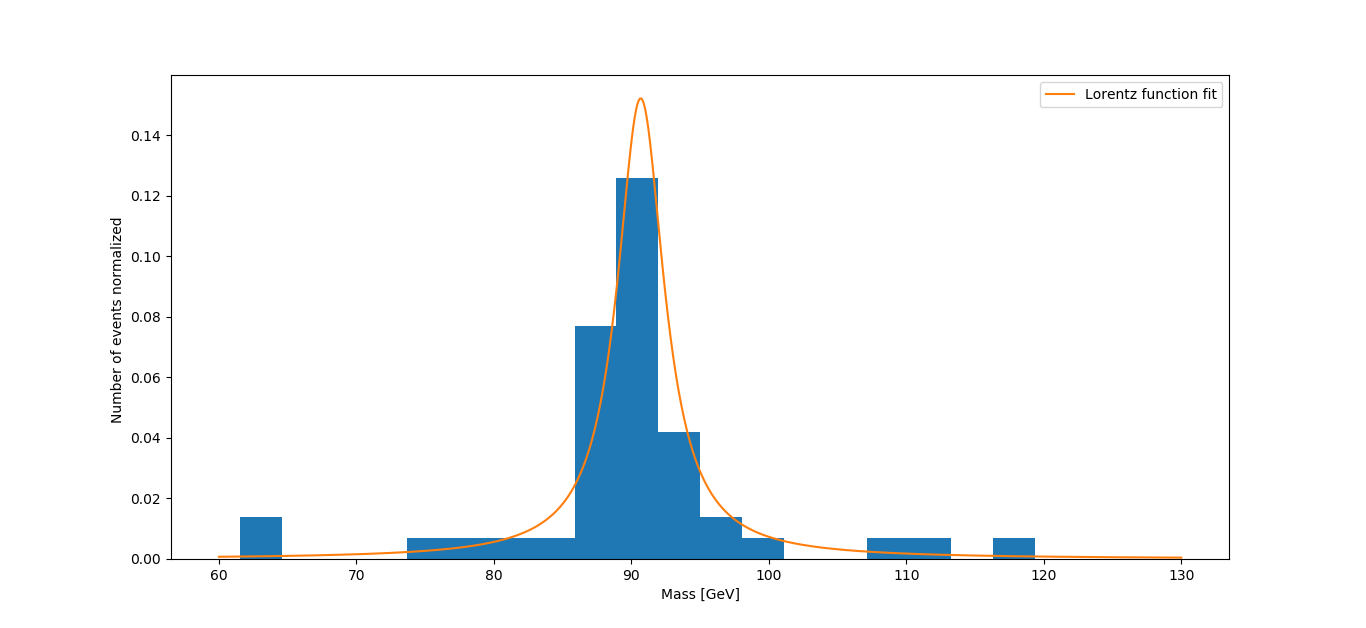
\includegraphics[width =.8\textwidth]{img/Zfit}
\caption{Fit with a Lorentz function over the area normalized histograms of Z decays}\label{fit}
\end{figure}


\section{Questions and exercise 4}
\begin{enumerate}
\item \textbf{When is a particle called a virtual particle?}

A particle that is more of a mathematical placeholder than a real, measurable particle. While there are particles that cannot be observed directly, e.g. due to their extremely short lifetime, they are still real. 

The main definition of a virtual particle from the point of view of quantum field theory is that virtual particles are ``off shell'', i.e., they don't satisfy the Einstein energy-momentum relationship; real particles on the other hand do and are thus called ``on shell''. This essentially means that a virtual particle doens't necessarily have to have it's ``real'' rest mass during it's lifetime.

 Thomson, M. (2013). "Modern particle physics". Cambridge University Press, ISBN 978-1107034266, pp. 117–119.
\item \textbf{How many of 100 Z bosons decay into quarks of any type? How many decay into muons? Consider that quarks come in three colours.}

According to \cite{Zdecay}, the experimentally measured decay channels of the Z boson are written down in table \ref{tab:z_boson_decays}. The sub-branches of leptons are almost equivalent, with a value of $3.366 \pm 0.007 \%$ for muons.

\begin{table}
\centering
    \begin{tabular}{l|r}
    \hline
    Neutrinos (all)       & $20.00 \pm 0.06 \%$   \\
    Charged leptons (all) & $10.097 \pm 0.003 \%$ \\
    Hadrons (all)         & $69.91 \pm 0.06 \%$   \\ \hline
    \end{tabular}
    \caption{Z boson decay channels, measured values. See \cite{XXX} for more details.}
    \label{tab:z_boson_decays}
\end{table}
 
\item \textbf{How is the lifetime $\tau$ connected to the Full width at half maximum (FWHM, \textit{Halbwertsbreite} in German)?}

The lifetime $\tau$ is indirectly proportional to the FWHM $\Gamma$ via the Heisnberg uncertainty relation in equation \ref{eq:heisenberg_uncertainty_lifetime}
\begin{equation}
\label{eq:heisenberg_uncertainty_lifetime}
\tau = \frac{\hbar}{\Gamma}
\end{equation}

\item \textbf{At the LHC, protons are accelerated to energies of $\SI{6.5}{\tera\electronvolt}$. How fast are they then (in units of $c$)? Calculate the relativistic gamma factor first. How much slower than photons are protons in the LHC for one round in the collider? What is the equivalent distance?}

The relativistic gamma factor can be calculated via
\begin{equation}
E = (\gamma -1)mc^2,
\end{equation}
using $m=\SI{938.272}{\mega\eV}/c^2$ as the proton mass. This yields a result of $\gamma = 6930$. Since $\gamma$ is defined via
\begin{equation}
\gamma = \frac{1}{\sqrt{1-\frac{v^2}{c^2}}},
\end{equation}
one can invert this equation to obtain ${v=0.999999989589 c}$.
\item \textbf{What magnetic field strength is needed to hold the protons in their track? Consider the radius in the curved sections to be $r = \SI{2.8}{\kilo\meter}$.}

In order for the proton to stay on a circular radius with $r=\SI{2.8}{\kilo\meter}$, the relativistic centripetal force
\begin{equation}
F_C = \frac{m \gamma v^2}{r}
\end{equation}
needs to be equal to the Lorentz force acting on a charged particle
\[
F_L = e (\vec{v} \times \vec{B})
\]
where $e$ is the elementary charge.
Since we are only interested in the scalar strength of the magnetic field, we can simplify the resulting equation to 
\[
B = \frac{m\gamma v}{r e}
\]
For our calculated values for $\gamma$ and $v$ we obtain a value of $B = \SI{7.746}{\tesla}$.
\item \textbf{How many decay channels are there for Z and W bosons, respectively?}

According to the Particle Data Group \cite{Zchannel},\cite{Wchannel}, there are 55 decay channels for the Z boson and 10 for the W boson. However, many of those are strongly suppressed and many are lumped together under one category. However, no better authoritarian document was found by us.
\end{enumerate}

\subsection{Excercise 4: Additional questions}

\begin{enumerate}
\item \textbf{Why is there a relativistic $\gamma$ factor in the formula for the relativistic centripetal force in question 5 of the lecture notes?}
Inside the LHC protons are accelerated to energies of roughly $\SI{6.5}{\tera\eV}$. This means we are in a highly relativistic regime and need to consider the relativistic mass $m= \gamma m_0$, where $m_0$ is the rest mass, in our formula. Thus the relativistic centripetal force is $F_{Cen} = m_0 \gamma v^2/r$.

\item \textbf{State a theoretical reason why there are about 10 times more W bosons than Z bosons in the production at LHC. For this, compare the reaction $q + \bar{q}' \to W \to \mu + \nu$ with $q + \bar{q} \to Z \to \mu + \mu$.}
\item \textbf{What is inconsistent in the notes about W boson production?}

In a pure proton-proton-collision, the only way valence quarks can combine into a W boson is via the combination $u + \bar{d} \to W^+$. In order for $W^-$ bosons to be produced as well, one would need an antiproton.
% not really sure about his answer
\item \textbf{In which cases is the error for the variable $G(x,y)$ with correlation and without correlation identical, considering error propagation of two variables $x$ and $y$ from a histogram?}
\item \textbf{Estimate how many Z decays one needs for the calculation of the literature value of the mean value of the Z mass.}
The literature value for the Z mass is given by $m(Z^0) = \SI{91187.6 \pm 2.1}{\mega/\eV}/c^2$, which is equivalent to an error of 0.231\%. In statistics, one can approximate the margin of error at the 95\% confidence level by
\[\text{margin of error} \approx \frac{0.98}{\sqrt{n}}\]
where $n$ is the sample size. For our error margin of 0.231\%, this means the sample size should be about 180000. 
\item \textbf{Discuss the difference between the numerical (Normal) mean value and the calculation of the mean value from using a fit function (a Lorentz function)?}
\item \textbf{Which three decay channels of the Higgs boson have you studied in this experiment? How many are there in total?}

The three decay channels we focused on were
\[H \to \gamma + \gamma\]
\[ H \to W^- W^+ \to \ell^+ + \nu + \ell^- + \bar{\nu}\]
\[ H \to ZZ \to 4 \ell\]
where $\gamma$ stands sfor a photon, $\ell$ for a lepton and $\nu$ for a neutrino. In total there are X decay channels for the Higgs boson.
\end{enumerate}
\begin{thebibliography}{99}

  \bibitem{masshiggs}
    G. Aad et al. (ATLAS Collaboration, CMS Collaboration) Phys. Rev. Lett. 114, 191803

  \bibitem{Zmass}
   J. Beringer et al. (Particle Data Group), PR D86, 010001 (2012)

   \bibitem{Zdecay}
   http://pdg.lbl.gov/2009/tables/rpp2009-sum-gauge-higgs-bosons.pdf

   \bibitem{ratio}
   The ATLAS Collaboration JHEP 1012(2010)060

   \bibitem{Zchannel}
   http://pdg.lbl.gov/2012/listings/rpp2012-list-z-boson.pdf
   \bibitem{Wchannel}
	http://pdg.lbl.gov/2012/listings/rpp2012-list-w-boson.pdf
\end{thebibliography}
\end{document}
